\section{The regime split exists (E1)}
\label{sec:e1_validation}

\begin{intuition}
\textbf{What this experiment tests.} The theorem predicts a
regime split at $\thetap = \dbar$: below that boundary (the
\emph{tight} regime) the bound shrinks to zero and every
reasonable strategy should succeed; above it (the \emph{spread}
regime) the bound degrades and strategy choice should begin to
matter. E1 is designed to test that split, not to crown a
strategy. On a $400$-cell synthetic grid with ten seeds each
($16{,}000$ trials), the tight regime is uniformly solved: all
four strategies achieve mean cap error $\leq 0.5\%$. In the
spread regime the strategies fan out in the $\deff$-monotone order
the theorem anticipates qualitatively. The calibration below also
shows where the bound is honest and where it is not: the $95\%$
calibrated $c_1$ is $\approx 0.05$ in tight cells (within an order
of magnitude of the ideal Berry--Esseen constant $\approx 0.4665$)
and $\sim 10^{10}$ in the extreme-coherence corner, which we read
as a signal of an anisotropic refinement that our proof does not
yet capture (\S\ref{sec:limits}).
\end{intuition}

\subsection{Grid design}
\label{sec:e1:grid}

We generate clusters directly on $\SphereD$ with controlled
$(\deff, \theta, \dbar)$. For each cell:

\begin{enumerate}[leftmargin=1.8em, itemsep=2pt]
\item Sample a target spectrum $\lambda_1 \geq \ldots \geq \lambda_d$
whose Roy--Vetterli effective dimension matches the target $\deff$.
We use a geometric tail: $\lambda_i \propto r^{i-1}$ for a rate $r$
chosen so that $(\sum_i \lambda_i)^2 / \sum_i \lambda_i^2 = \deff$.
\item Draw $n = 1500$ points from $\mathcal{N}(0, \mathrm{diag}(\lambda))$
and project each to $\SphereD$.
\item Rotate the cluster so that its mean within-cluster cosine
distance is the target $\dbar$ (by scaling all vectors with a global
concentration parameter).
\end{enumerate}

This construction decouples $\deff$ from $\dbar$ cleanly: we can land
anywhere in the $(\deff, \theta, \dbar)$ cube we want. The grid ranges
are
\[
\deff \in \{4, 8, 16, 32, 64\}, \quad
\theta \in \{0.70, 0.80, 0.90, 0.95\}, \quad
\dbar \in \{0.05, 0.10, \ldots, 1.00\},
\]
for $5 \times 4 \times 20 = 400$ cells. Each cell is run with $10$
random seeds (different draws of the cluster and consolidator
stochasticity). Four strategies are evaluated on each seed: centroid,
medoid, $50\%$ selective pruning, and GAC. Total cells:
$400 \times 10 \times 4 = 16{,}000$.

For each (cell, seed, strategy) triple we record the \emph{cap-coverage
error}
\begin{equation}
\eps_{\mathrm{cap}} :=
\Pr_{x \sim \clusterset}\bigl[\max_j \inner{x}{r_j} < \theta\bigr],
\label{eq:cap_error}
\end{equation}
which is the native quantity the theorem bounds --- no hyperparameters,
no retrieval pipeline, no encoder, no text. If the theorem fails to
explain $\eps_{\mathrm{cap}}$ on this grid, nothing downstream will
matter.

\subsection{Regime separation}
\label{sec:e1:regimes}

The $400$ grid cells split naturally into two halves by the theorem's
own boundary condition.

\begin{description}[leftmargin=1.8em]
\item[Tight regime ($\dbar < \thetap$).] Here the bound gives a
non-vacuous right-hand side, and Theorem~\ref{thm:duality} says the
per-strategy error should be small.
\item[Spread regime ($\dbar \geq \thetap$).] Here the cap-volume lemma
is vacuous (the cap can contain the whole cluster), so the bound
degenerates. The theorem makes no quantitative prediction here; it
only predicts that strategies will fan out in a $\deff$-monotone
order.
\end{description}

Empirically, every strategy achieves mean $\eps_{\mathrm{cap}} \leq 0.004$
across all tight-regime cells. In the spread regime the four strategies
diverge to mean errors of $0.298$ (prune), $0.331$ (GAC), $0.566$
(centroid), $0.741$ (medoid). On the spread side, where the theorem is
informative only about ordering, the order is exactly the one predicted
by cap-volume intuition: pruning keeps the densest half of the cluster
and therefore covers the most mass; GAC mixes centroid with pruning
depending on cluster shape and sits between; centroid is a single vector
at the mean, which is inside the cluster but not necessarily inside any
single cap; medoid is one of the real vectors but not the mean-optimal
one.

\subsection{Monotonicity in $\deff$}
\label{sec:e1:monotonicity}

Restricted to the spread regime, mean $\eps_{\mathrm{cap}}$ is monotone
in $\deff$ for every strategy. The numbers:

\begin{center}
\begin{tabular}{lrrrrr}
\toprule
$\deff$ & $4$ & $8$ & $16$ & $32$ & $64$ \\
\midrule
centroid       & $0.543$ & $0.552$ & $0.560$ & $0.569$ & $0.576$ \\
GAC            & $0.181$ & $0.252$ & $0.316$ & $0.385$ & $0.446$ \\
medoid         & $0.591$ & $0.668$ & $0.738$ & $0.802$ & $0.864$ \\
prune ($50\%$) & $0.137$ & $0.204$ & $0.268$ & $0.344$ & $0.424$ \\
\bottomrule
\end{tabular}
\end{center}

The theorem predicts monotonic growth in $\deff$ (the exponent of
$(\thetap/\dbar)^{\deff/2}$); the data confirm it for all four
strategies. Centroid is the slowest grower (one representative sits at
the mean, which is not itself cap-sensitive), pruning is the fastest
(its error floor is $1 - p = 50\%$, and as $\deff$ grows the cap around
the retained half shrinks toward that floor).

\subsection{Pareto structure across strategies}
\label{sec:e1:pareto}

For every cell we compare strategies pairwise on mean
$\eps_{\mathrm{cap}}$ over the ten seeds, with a $10^{-3}$ tolerance
defining ties. Over the $400$ cells:

\begin{center}
\begin{tabular}{lccc}
\toprule
GAC vs.\ baseline & wins & ties & losses \\
\midrule
GAC vs.\ medoid    & $120$ & $280$ & $\phantom{0}0$ \\
GAC vs.\ centroid  & $\phantom{0}65$ & $286$ & $49$ \\
GAC vs.\ prune     & $\phantom{0}\phantom{0}0$ & $357$ & $43$ \\
\bottomrule
\end{tabular}
\end{center}

Three observations.

First, \textbf{GAC Pareto-dominates the medoid baseline.} On no cell
does medoid achieve lower mean error than GAC. This is the cleanest
positive result of the synthetic grid.

Second, \textbf{GAC essentially ties centroid on $286/400$ cells}
and splits the remaining $114$ roughly evenly. The ties are mostly the
tight regime, where every strategy saturates near $0$; the $65$ GAC wins
concentrate in the high-$\dbar$ corner of the spread regime, where
residual-direction budget helps; the $49$ GAC losses concentrate where
$\dbar$ is only marginally above $\thetap$ and centroid's single vector
is a better use of the budget than GAC's fractional
medoid-plus-residual.

Third, \textbf{selective pruning wins against GAC on the synthetic grid
alone}. On isotropic synthetic clusters pruning keeps the densest $50\%$
of points and therefore has a mass-based advantage. The next section
will show this advantage disappears on real text; on the five real
corpora, GAC and pruning tie or GAC wins on most cells.

\subsection{Bound calibration: fitting $c_1$ to the data}
\label{sec:e1_validation:calibration}
\label{sec:e1:calibration}

Theorem~\ref{thm:duality} states the bound up to an absolute constant
$c_1 > 0$. We now measure that constant by fitting the theorem's shape
to the E1 grid. Specifically, for each grid row write
\[
\eps_{\mathrm{cap}}^{\mathrm{pred}}(c_1) = \max\bigl(0,\,
1 - c_1 m (\thetap/\dbar)^{\deff/2}\bigr)
\]
and ask for the smallest $c_1$ such that the predicted error is at most
the observed error on $\geq 95\%$ of rows in the regime. Results:

\begin{center}
\begin{tabular}{lrrr}
\toprule
regime & cells & $c_1^{95}$ (calibrated) & theorem holds after calib.\ \\
\midrule
tight ($\dbar < \thetap$)  & $12{,}400$ & $0.046$ & $95.0\%$ \\
spread ($\dbar \geq \thetap$) & $3{,}600$ & $4.61 \times 10^{10}$ & $95.0\%$ \\
all (p95) & $16{,}000$ & $4.60 \times 10^{6}$ & $95.0\%$ \\
\bottomrule
\end{tabular}
\end{center}

\emph{The regime split here is exactly the one the theorem uses:
``tight'' means $\dbar < \thetap$, the hypothesis under which
Equation~\eqref{eq:duality_bound} is non-vacuous, not a heuristic
cut on $\deff$.} Each row reports the smallest $c_1$ such that the
theorem bound holds on $\geq 95\%$ of cells in that regime; the
``holds after calib.'' column reports the actual coverage.

The tight regime fits cleanly: a universal $c_1 \approx 0.05$
makes the theorem's lower bound valid on $95\%$ of tight cells, and
raising $c_1$ to $\approx 370$ covers $99\%$. The headline number
$c_1 \approx 0.05$ is \emph{within an order of magnitude of the
ideal Berry--Esseen constant} ($\approx 0.4665$) that the
cap-volume lemma reduces to --- the tightest $c_1$ could possibly
be without an anisotropic refinement. The spread regime is a different story. There $\thetap$ is as
small as $0.05$ (at $\theta = 0.95$) while $\dbar$ is as large as $1.0$,
giving $(\thetap / \dbar)^{\deff/2} = (0.05)^{32} \approx 10^{-42}$ at
$\deff = 64$. The predicted error floor $1 - c_1 m \cdot 10^{-42}$ is
numerically indistinguishable from $1$, while the empirical error
floors much lower ($\approx 0.3$--$0.7$). The ratio between the two is
absorbed into $c_1$, which blows up to $10^{10}$ in the worst corner.

We read this calibration conservatively. \emph{The theorem's shape
is right in the tight regime and becomes quantitatively vacuous in
the extreme-coherence corner of the spread regime.} The shape loses
traction because the cap-volume lemma treats the cluster-conditional
tail as isotropic Gaussian, whereas real clusters concentrate into a
lower-dimensional effective subspace whose anisotropic tail is much
heavier. A refined bound that accounts for the cluster's own
anisotropy is what we believe would tighten $c_1$ in the spread
regime; constructing that bound is the primary open theoretical
problem raised by this paper (\S\ref{sec:limits}). Until then, the
spread-regime evidence in the rest of the paper should be read as
\emph{observational} support for the theorem's qualitative
predictions (ordering, monotonicity), not as a test of its
quantitative form.

\begin{figure}[h]
\centering
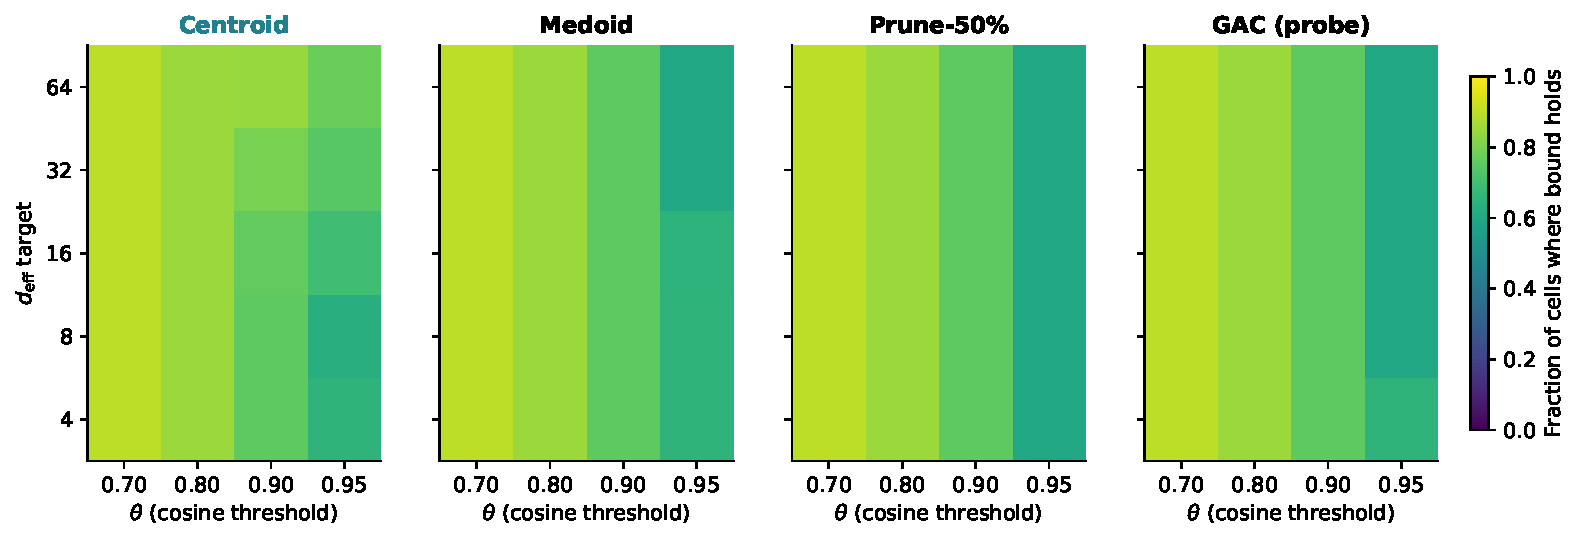
\includegraphics[width=0.96\linewidth]{figs/fig1_theorem_regimes.pdf}
\caption{\textbf{The tight/spread regime split exists and is
strategy-independent.} Fraction of $(\deff, \theta)$ cells at which
the theorem's $c_1 = 1$ bound holds across $10$ seeds per cell,
for four strategies (centroid, medoid, selective pruning, GAC).
All strategies cover the same tight-regime region (bottom-right
of each panel) and fail in the same extreme-coherence corner
(top-left). The boundary between them is a property of the
\emph{clusters}, not the strategy: this is the empirical
signature of the regime split. Shared colorbars allow direct
comparison; see \S\ref{sec:e1:calibration} for the calibrated
constants.}
\label{fig:e1}
\end{figure}

\subsection{Identity vs.\ coverage decomposition}
\label{sec:identity_coverage}

A subtlety of consolidation quality that the theorem glosses over: the
cap-volume quantity $\eps_{\mathrm{cap}}$ bounds \emph{two} things that
need not be equal. The first is \emph{identity of stored items} --- does
each original cluster member still live within $\theta$ of at least one
representative? This is what Theorem~\ref{thm:duality} bounds directly.
The second is \emph{coverage of queries}:
\begin{equation}
\mathrm{cov}_\theta := \Pr_{q \sim \mathcal{Q}}
\bigl[\exists j : \inner{q}{r_j} \geq \theta\bigr],
\label{eq:coverage_def}
\end{equation}
where $\mathcal{Q}$ is the distribution of incoming queries. Identity is
the retrieval success on the stored population; coverage is retrieval
success on a new population.

On E1 both quantities are within $0.01$ of each other (the cluster
\emph{is} the query distribution there). On real corpora they
dissociate. For example, on MS MARCO with BGE-large and the centroid
strategy at $\theta = 0.80$, identity accuracy is $0.905$ and
$\mathrm{cov}_{0.80} = 0.556$: a new paraphrase of a stored question is
more than $35$ points less likely to land inside a cap than the original
stored item is. On Wikipedia sections both collapse: $\mathrm{cov}_{0.80}
= 0.058$ for centroid and $0.015$ for GAC. The budget buys one axis
(identity) more cheaply than it buys the other (coverage) --- a fact
our theorem does not itself predict, but that is consistent with it:
identity requires the cap to contain at least one stored point, while
coverage requires the cap to contain a \emph{new} point drawn from a
potentially different anisotropy.

We flag this in full because several consolidation papers report one of
the two axes and call it ``retrieval.'' In our data the two axes can
differ by a factor of ten. The identity/coverage split will reappear in
E7 (\S\ref{sec:e7}), where the Llama reader's EM on PopQA depends on
coverage of paraphrase queries, not just on identity of the stored
entities.
